% ######################################################################################################################
%         Introduction
% ######################################################################################################################

\chapter{Introduction}
\label{ch:Introduction}

% ######################################################################################################################
%         Background and Motivation
% ######################################################################################################################

\section{Background and Motivation}
\label{ch:Introduction:sec:Motivation}

The concept of evolution is the cornerstone of modern biology \cite{Dobzhansky1973}.
% \secref{ch:Foundations:sec:EvolutionGenetics}
All life on earth descends from a common ancestor and continuously evolves over generations,
which leads to a diversification of biological species.
The resulting branching pattern of the evolutionary relationships between species
is the key for unraveling many biological questions.
These evolutionary relationships are described by \emph{phylogenetic trees}
(\secref{ch:Foundations:sec:TreeOfLife}),
which are important in both basic \cite{Misof2014,Jarvis2014,Zanne2014} and
applied research \cite{Futuyma1995,Hendry2011,Schwartz2017}.

Characteristics and traits of biological species are inherited via their DNA
(\secref{ch:Foundations:sec:EvolutionGenetics}).
DNA data is hence often used for inferring a phylogenetic tree for a set of species
(\secref{ch:Foundations:sec:MLTreeInference}).
In order to conduct such analyses, the DNA has to be sequenced,
that is, it has to be ``read'' into some human-accessible format,
typically in form of a sequence of characters
(\secref{ch:Foundations:sec:SequenceAnalysis}).
In recent decades, the throughput of sequencing technologies increased,
while at the same time, the cost decreased faster than Moore's law,
as shown in \figref{fig:sequencing_costs}.
Currently, the sequencing capacity doubles roughly every seven months \cite{Stephens2015}.
This lead to a ``tsunami'' of sequence data,
which constitutes a challenge for computational analyses of these data.
% computational biology

\begin{figure}[hbt]
    \centering
    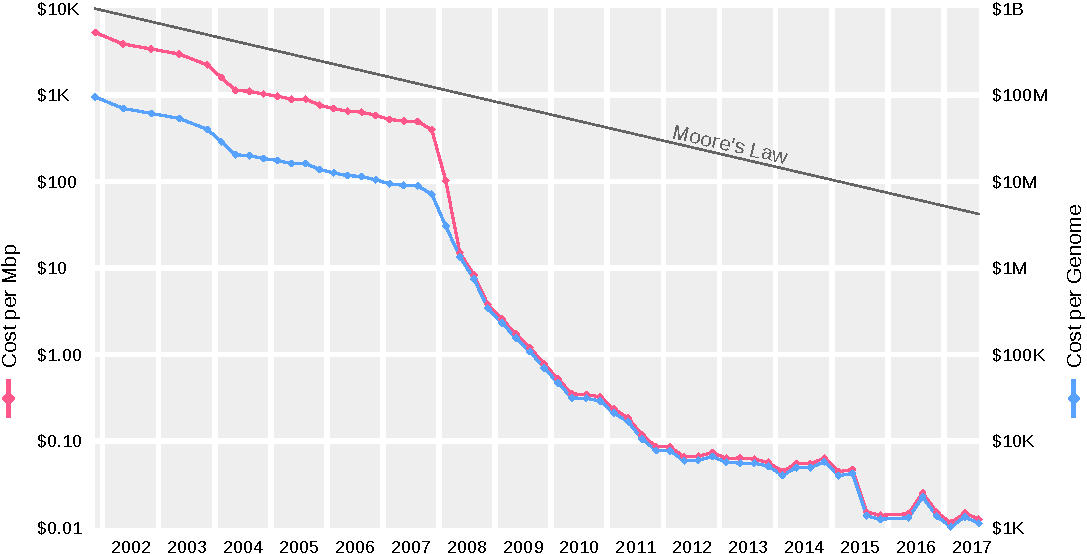
\includegraphics[width=\linewidth]{sequencing_costs.pdf}
    \caption[Sequencing costs per Mbp and per genome]{
        \textbf{Sequencing costs per Mbp and per genome.}
        The cost for DNA sequencing have decreased substantially in the past 15 years.
        The Figure shows the cost per mega-basepair (Mbp) of DNA (red line, left y-axis)
        as well as the cost per human-sized genome of $\approx$\,\num{3}\,Gbp (blue line, right y-axis).
        A basepair represents one character in the DNA.
        Note the logarithmic scaling of the y-axes.
        For comparison, Moore's law \cite{Moore1965} is shown.
        The particularly steep decrease in the beginning of 2008 is caused by
        the adoption of novel (next-generation) sequencing technologies in sequencing centers,
        see \secref{ch:Foundations:sec:SequenceAnalysis:sub:GenomeSequencing}.
        Source: Image based on data from \cite{Wetterstrand2018}.
%         \url{https://www.genome.gov/sequencingcosts/}
%         \url{https://www.genome.gov/sequencingcostsdata/}
    }
    \label{fig:sequencing_costs}
\end{figure}

In particular, these high-throughout technologies allow to directly sequence DNA contained in samples
that have been extracted from environments such as water, soil, or the human gut.
This results in so-called \emph{metagenomic} sequences,
i.e., anonymous DNA sequences from the (microbial) organisms that were present in the environmental sample.
A key question in the analysis of such data is to determine the evolutionary relationships of the sequences.
While these DNA sequences can hypothetically be used to infer phylogenetic trees from scratch,
this approach is limited by several theoretical and practical difficulties:
For instance, typical metagenomic samples contain too many, and too short, sequences
for a feasible and reliable tree inference.

One approach to tackle this issue is the so-called \emph{phylogenetic placement} \cite{Matsen2010,Berger2011},
of metagenomic sequences into a given phylogenetic tree (\secref{ch:Foundations:sec:PhylogeneticPlacement}).
Phylogenetic placement methods classify a set of \emph{query sequences}
into the context of known evolutionary relationships, provided in form of a \emph{reference tree}.
While this information already represents biological knowledge \emph{per se},
it can also be used for further downstream analyses \cite{Matsen2011a}.
Although such phylogeny-aware methods offer large potential for sequence data analysis and interpretation,
the research in this field is quite young and not many such analysis methods have been developed.

An important task prior to conducting phylogenetic placement of metagenomic sequences is to obtain a suitable
reference phylogenetic tree that captures the biological diversity of the species to be placed.
The assembly of a set of reference sequences from biological databases that can be used to infer such a tree
is typically a manual process, and hence both labor-intensive and potentially error-prone.
This might detain researchers from employing phylogenetic placement in the first place.

Furthermore, while the existing downstream methods for phylogenetic placement
(introduced in \secref{ch:Foundations:sec:PhylogeneticPlacement:sub:ExistingMethods})
allow for in-depth interpretation and visualization of the data,
they were not developed with a particular focus on large-scale studies comprising many thousand environmental samples.
For large datasets, these methods might provide too much detail,
making it hard to interpret results, to spot patterns and clusters in the data,
and to discover correlations with per-sample meta-data.

Lastly, the problem of scalability to large datasets does not only affect the methods themselves.
Because of the ever growing amount of sequence data,
scalability is becoming an issue for the software pipelines as well.
State-of-the-art phylogenetic placement implementations can process billions of sequences within a few hours \cite{Barbera2018}.
Methods for handling and analyzing the data, in particular phylogenetic placement data,
hence require efficient and scalable software implementations.

% ######################################################################################################################
%         Objective and Contribution
% ######################################################################################################################

% \section{Objective and Contribution}
% \label{ch:Introduction:sec:ObjectiveContribution}

\section{Contribution and Overview}
\label{ch:Introduction:sec:ContributionOverview}

This thesis makes several contributions to the field of computational phylogenetics,
specifically for conducting phylogenetic placement and analyzing the resulting data.
In particular, we introduce multiple novel methods to overcome the issues and limitations described above.
The methods were already described in two peer-reviewed publications \cite{Czech2018,Czech2018a},
and their data and scripts were made available at \url{http://github.com/lczech/placement-methods-paper}.
% phat \cite{Czech2018}
% vis clust \cite{Czech2018a}
% \citeauthor{Czech2018} and \citeauthor{Czech2018a} and \citeauthor{Czech2018,Czech2018a}

Firstly, we describe an automated approach for obtaining suitable reference trees for phylogenetic placement,
as well as pre-processing pipelines to accelerate and enable
phylogenetic placement of large metagenomic datasets (\chpref{ch:AutomaticTrees}).
Secondly, we introduce methods to visualize such large datasets
in order to detect patterns within the data and correlations with per-sample meta-data (\chpref{ch:Visualization}).
Lastly, we present an approach for clustering metagenomic samples (\chpref{ch:Clustering}),
measuring similarity between samples in terms of the species diversity they contain.

Apart from the two publications on which this thesis is based,
we reviewed several software tools for visualizing phylogenetic trees \cite{Czech2017}.
In this publication, we investigated whether certain types of per-branch and per-node meta-data of phylogenetic trees
were correctly displayed in \num{20} tools, particularly when first modifying the tree topology.
We found that most of the tested tools had some kind of issue or undocumented behavior and
did not properly support the \fileformat{Newick} file format for phylogenetic trees.
We also showed that this already has affected trees published in peer-reviewed journals.

In addition to these theoretical projects, we also helped in several empirical data analysis studies
by conducting established analysis methods as well as prototypes of our novel methods.
In particular, we ran the phylogenetic analyses for a study of \num{154} locations
in neotropical rainforest soils \cite{Mahe2017}.
The study found that the microbial diversity in these soils is dominated by protistic parasites.
For this project, we developed prototypes of our multilevel placement approach
(\secref{ch:AutomaticTrees:sec:Methods:sub:MultilevelPlacement})
as well as of some visualization techniques (\secref{ch:Visualization:sec:Motivation}).

Further data analysis studies that we contributed to include the 1KITE project \cite{Misof2014} (\url{http://1kite.org}),
where we helped to conduct phylogenetic tree reconstructions for a diverse set of \num{1500} insects,
as well as a study of \taxonname{Microsopirida} and \taxonname{Cryptomycota} \cite{Bass2018a},
were we contributed phylogenetic placement analyses
in order to resolve some branches in the phylogenetic tree of these groups of microbial \taxonname{Eukaryotes}.
\todo{Mention the current projects as well?:}
An ongoing large-scale endeavor is the UniEuk project \cite{Berney2017},
which aims to become a unified reference database for the \taxonname{Eukaryotes},
and to which we provided consultancy and helped in planning workflows and pipelines.
In a current empirical project, we develop tools for analyzing a dataset of microbial \taxonname{Eukaryotes},
with the aim of showing that novel sequencing technologies that yield longer sequences per run
can improve taxonomic and phylogenetic analyses compared to other sequencing technologies.
Lastly, we are currently working on an empirical dataset of \taxonname{Dinoflagellates},
where we also conducted phylogenetic placement analyses.

In the course of developing our novel methods, we implemented them in \texttt{C++},
and provide the resulting code in our open-source library \toolname{genesis} (\url{https://github.com/lczech/genesis}).
Apart from our novel methods, the library provides efficient re-implementations of existing methods \cite{Matsen2010},
which are faster than the original implementation by orders of magnitude.
Furthermore, the library also implements a multitude of data structures and functions for working with
phylogenetic placements, genetic sequences, phylogenetic trees, taxonomies, and many other data types,
as well as a plethora of auxiliary functions for tasks such as visualizations, statistical evaluations, and data storage.
Moreover, in order to also offer a user-friendly command line interface for the most important novel and established methods,
we developed the open-source tool \toolname{gappa} (\url{https://github.com/lczech/gappa}),
which stands for ``Genesis Applications for Phylogenetic Placement Analysis''.
It is intended for researchers who want to conduct analyses using our methods,
and internally uses the \toolname{genesis} library for its computations.
For details on the software implementations, see \appref{ch:PipelineImplementation}.
\todo{ref to genesis/gappa paper?!}

Moreover, we contributed to several other open-source software projects.
We helped to develop an efficient approach for merging so-called \emph{paired-end reads} \cite{Flouri2017}
and provided SIMD (single instruction, multiple data) implementations using \texttt{SSE} and \texttt{AVX} instructions
to accelerate the merging algorithms.
Again for acceleration, we implemented a custom \texttt{\acs{MPI}} wrapper for \toolname{PaPaRa 2.0} \cite{Berger2011a,Berger2012},
a tool for aligning query sequences to a given reference alignment and phylogenetic tree,
which we made available at \url{https://github.com/lczech/papara_nt}.
During the development of the recent high-performance re-implementation of the phylogenetic placement algorithm
in \toolname{EPA-ng} \cite{Barbera2018}, we helped with software design decisions and implementation details questions,
and our \toolname{genesis} library was used in the project.
We also helped with the implementation and acceleration of a novel quartet-based method to accurately and robustly
measure incongruence between phylogenetic trees \cite{Zhou2017},
where again the \toolname{genesis} library was used.
Furthermore, we provided code for the sequence clustering tool \toolname{swarm} \cite{Mahe2014,Mahe2015},
which was the basis for accelerating the software by almost an order of magnitude on large datasets,
and which will be part of the upcoming version~3 of \toolname{swarm}.
Lastly, we are currently working on \toolname{scrapp},
a pipeline that combines several tools of our lab, such as
\toolname{EPA-ng} \cite{Barbera2018}, \toolname{ParGenes} \cite{Morel2018}, and \toolname{mPTP} \cite{Kapli2017},
in order estimate the species diversity in metagenomic sequence samples based on phylogenetic placement data;
see also \chpref{ch:ConclusionOutlook}.
\todo{check what we write there about scrapp}

A full list of our publications is also available in \appref{ch:Publications}.

The remainder of this thesis is structured as follows.
First, we introduce the general concepts and existing methods
of computational phylogenetics and phylogenetic placement in \chpref{ch:Foundations}.
Then, in Chapters \ref{ch:AutomaticTrees}--\ref{ch:Clustering}, we describe the aforementioned novel methods
for conducting and analyzing phylogenetic placements.
Finally, we conclude and discuss future work in \chpref{ch:ConclusionOutlook}.

% tree clustering workshop?

% ######################################################################################################################
%         Structure and Overview
% ######################################################################################################################

% \section{Structure and Overview}
% \label{ch:Introduction:sec:StructureOverview}

\todo{check that the url and access date of all online sources are present in bibliography!}

% \todo{I used a few public domain images from wikipedia as sources, and modified them as needed. make sure that this is okay.}

\todo{search for all abbreviations used and add them to the acro list. also, check Pierre's MA, and Alexey's and Andre's Diss for needed acronyms!}
\todo{list of acronyms!} see andre, add MB/GB, PCA,
BV, TO, HMP, etc

\todo{sort acronyms alphabetically}
\todo{make acronyms all in same capitalization}

\todo{unify table and figure caption capitalization}

\todo{unify citep cite}

\todo{more workflow flow charts?}

\todo{add pdf bookmarks for frontmatter chapters}
